% Chapter 1 (from pres-main tex file)
% New Trends in Research
% Author: Javier Reyes

\subsection{Zynqberry 726}

\begin{frame}
	\frametitle{Zynqberry 726}
	Single Board Computer: \pause
	\begin{itemize}
		\item Xilinx Zynq-7010 device. \pause
		\item Raspberry Pi Form Factor. \pause
		\item Board-mounted peripherials:
		\begin{itemize}
			\item 16 MB Flash, 512 MB DDR3L SDRAM, 4xUSB 2.0, 10/100 Mbit Ethernet RJ45, Micro SD card slot, HDMI connector, DSI display connector, CSI-2 camera connector, HAT header with 26 IO, 3.5 mm stereo audio socket, Micro-USB (power, USB-UART, JTAG).
		\end{itemize}
	\end{itemize}
\end{frame}

\begin{frame}
	\frametitle{Zynqberry 726}
	\begin{columns}
		\begin{column}{0.4\textwidth}
			\begin{figure}
				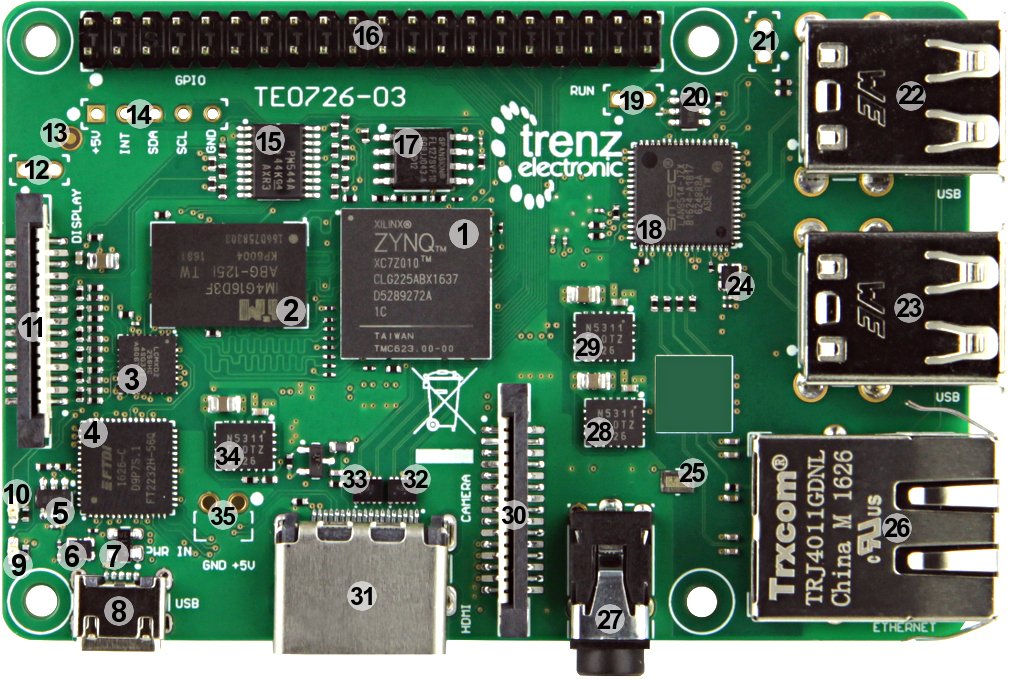
\includegraphics[width=\textwidth]{zynqberry-top.png}
				\caption{Zynqberry 726 board.}\label{fig:zynqberry-top}
			\end{figure}
		\end{column} \pause
		\begin{column}{0.5\textwidth}
			\begin{figure}
				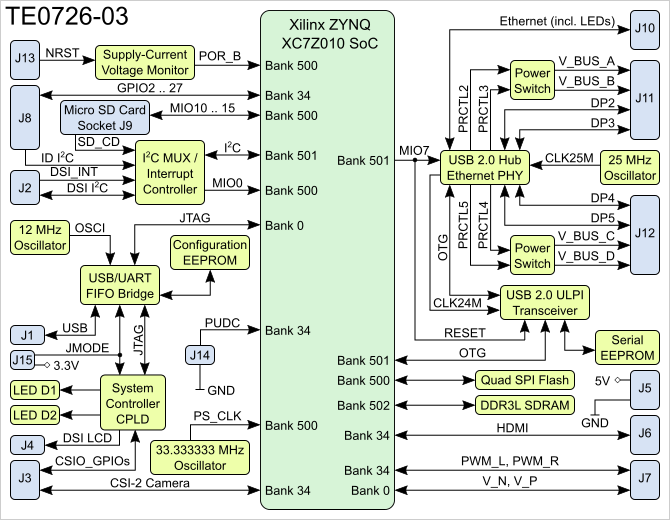
\includegraphics[width=\textwidth]{zynq-block-diagram.png}
				\caption{Zynqberry 726 block diagram \cite{zynq-trm}.}\label{fig:zynq-block-diagram}
			\end{figure}
		\end{column}
	\end{columns}
\end{frame}

\subsection{Zynq XC7Z010}

\begin{frame}
	\frametitle{Zynq XC7Z010}
	System on Chip (SoC) device from the Xilinx Zynq 7000 family: \pause
	\begin{itemize}
		\item Dual-core ARM Cortex A9 processor. \pause
		\item 28 nm Xilinx Artix-7 programmable logic device. \pause
		\item Integrated memory mapped Peripherals:
		\begin{itemize}
			\item 2x USB 2.0, 2x Gigabit Ethernet, 2x SD, 2x UART, 2x CAN 2.0B, 2x I2C, 2x SPI, 32b GPIO.
		\end{itemize}
	\end{itemize}
\end{frame}

\begin{frame}
	\frametitle{Zynq 7000 family}
	\begin{figure}
		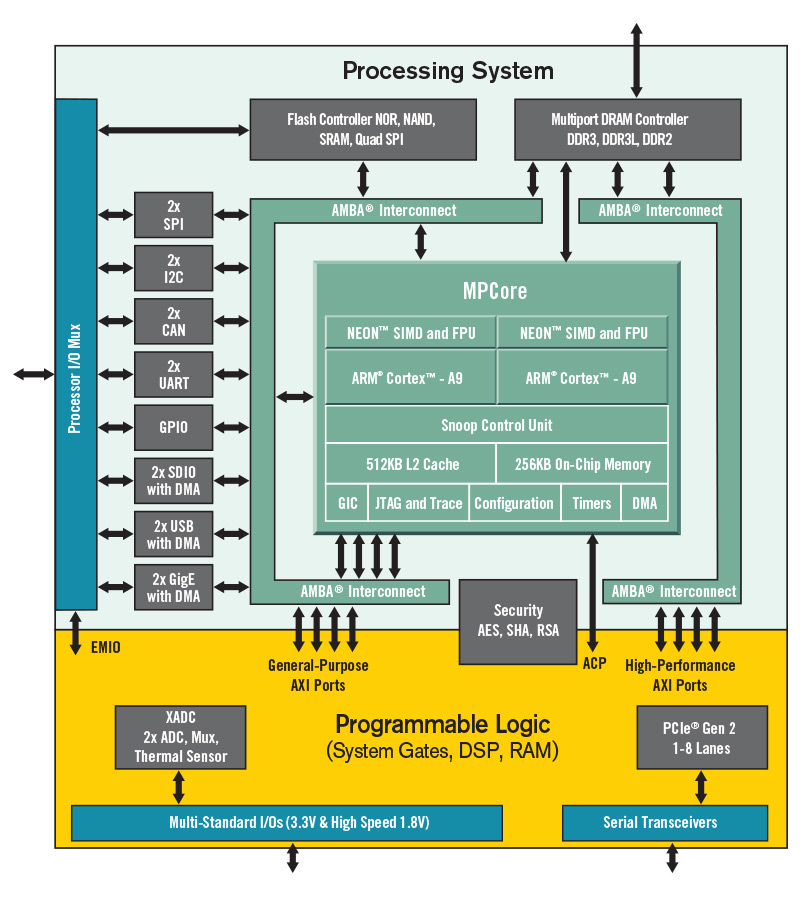
\includegraphics[width=0.5\textwidth]{zynq-arch-diag.png}
		\caption{Zynq-7000 device family architecture.}\label{fig:zynq-arch-diag}
	\end{figure}
\end{frame}

\begin{frame}
	\frametitle{Zynqberry Vs. Zynq 7Z010}
	The PS includes two Ethernet controllers, but the PHY attached to the Ethernet port on the board is connected to a USB-to-Ethernet interface.
	\vfill \pause
	\begin{alertblock}{Constraint}
		The hardware design needs to use the USB controller for any Ethernet communication.
	\end{alertblock}
\end{frame}